\documentclass[twoside]{book}

% Packages required by doxygen
\usepackage{fixltx2e}
\usepackage{calc}
\usepackage{doxygen}
\usepackage[export]{adjustbox} % also loads graphicx
\usepackage{graphicx}
\usepackage[utf8]{inputenc}
\usepackage{makeidx}
\usepackage{multicol}
\usepackage{multirow}
\PassOptionsToPackage{warn}{textcomp}
\usepackage{textcomp}
\usepackage[nointegrals]{wasysym}
\usepackage[table]{xcolor}

% Font selection
\usepackage[T1]{fontenc}
\usepackage[scaled=.90]{helvet}
\usepackage{courier}
\usepackage{amssymb}
\usepackage{sectsty}
\renewcommand{\familydefault}{\sfdefault}
\allsectionsfont{%
  \fontseries{bc}\selectfont%
  \color{darkgray}%
}
\renewcommand{\DoxyLabelFont}{%
  \fontseries{bc}\selectfont%
  \color{darkgray}%
}
\newcommand{\+}{\discretionary{\mbox{\scriptsize$\hookleftarrow$}}{}{}}

% Page & text layout
\usepackage{geometry}
\geometry{%
  a4paper,%
  top=2.5cm,%
  bottom=2.5cm,%
  left=2.5cm,%
  right=2.5cm%
}
\tolerance=750
\hfuzz=15pt
\hbadness=750
\setlength{\emergencystretch}{15pt}
\setlength{\parindent}{0cm}
\setlength{\parskip}{3ex plus 2ex minus 2ex}
\makeatletter
\renewcommand{\paragraph}{%
  \@startsection{paragraph}{4}{0ex}{-1.0ex}{1.0ex}{%
    \normalfont\normalsize\bfseries\SS@parafont%
  }%
}
\renewcommand{\subparagraph}{%
  \@startsection{subparagraph}{5}{0ex}{-1.0ex}{1.0ex}{%
    \normalfont\normalsize\bfseries\SS@subparafont%
  }%
}
\makeatother

% Headers & footers
\usepackage{fancyhdr}
\pagestyle{fancyplain}
\fancyhead[LE]{\fancyplain{}{\bfseries\thepage}}
\fancyhead[CE]{\fancyplain{}{}}
\fancyhead[RE]{\fancyplain{}{\bfseries\leftmark}}
\fancyhead[LO]{\fancyplain{}{\bfseries\rightmark}}
\fancyhead[CO]{\fancyplain{}{}}
\fancyhead[RO]{\fancyplain{}{\bfseries\thepage}}
\fancyfoot[LE]{\fancyplain{}{}}
\fancyfoot[CE]{\fancyplain{}{}}
\fancyfoot[RE]{\fancyplain{}{\bfseries\scriptsize Generated by Doxygen }}
\fancyfoot[LO]{\fancyplain{}{\bfseries\scriptsize Generated by Doxygen }}
\fancyfoot[CO]{\fancyplain{}{}}
\fancyfoot[RO]{\fancyplain{}{}}
\renewcommand{\footrulewidth}{0.4pt}
\renewcommand{\chaptermark}[1]{%
  \markboth{#1}{}%
}
\renewcommand{\sectionmark}[1]{%
  \markright{\thesection\ #1}%
}

% Indices & bibliography
\usepackage{natbib}
\usepackage[titles]{tocloft}
\setcounter{tocdepth}{3}
\setcounter{secnumdepth}{5}
\makeindex

% Hyperlinks (required, but should be loaded last)
\usepackage{ifpdf}
\ifpdf
  \usepackage[pdftex,pagebackref=true]{hyperref}
\else
  \usepackage[ps2pdf,pagebackref=true]{hyperref}
\fi
\hypersetup{%
  colorlinks=true,%
  linkcolor=blue,%
  citecolor=blue,%
  unicode%
}

% Custom commands
\newcommand{\clearemptydoublepage}{%
  \newpage{\pagestyle{empty}\cleardoublepage}%
}

\usepackage{caption}
\captionsetup{labelsep=space,justification=centering,font={bf},singlelinecheck=off,skip=4pt,position=top}

%===== C O N T E N T S =====

\begin{document}

% Titlepage & ToC
\hypersetup{pageanchor=false,
             bookmarksnumbered=true,
             pdfencoding=unicode
            }
\pagenumbering{alph}
\begin{titlepage}
\vspace*{7cm}
\begin{center}%
{\Large Projeto 2 Unidade 2 }\\
\vspace*{1cm}
{\large Generated by Doxygen 1.8.14}\\
\end{center}
\end{titlepage}
\clearemptydoublepage
\pagenumbering{roman}
\tableofcontents
\clearemptydoublepage
\pagenumbering{arabic}
\hypersetup{pageanchor=true}

%--- Begin generated contents ---
\chapter{Hierarchical Index}
\section{Class Hierarchy}
This inheritance list is sorted roughly, but not completely, alphabetically\+:\begin{DoxyCompactList}
\item \contentsline{section}{Point}{\pageref{class_point}}{}
\item \contentsline{section}{Poligono}{\pageref{class_poligono}}{}
\begin{DoxyCompactList}
\item \contentsline{section}{Retangulo}{\pageref{class_retangulo}}{}
\end{DoxyCompactList}
\end{DoxyCompactList}

\chapter{Class Index}
\section{Class List}
Here are the classes, structs, unions and interfaces with brief descriptions\+:\begin{DoxyCompactList}
\item\contentsline{section}{\mbox{\hyperlink{class_circulo}{Circulo}} }{\pageref{class_circulo}}{}
\item\contentsline{section}{\mbox{\hyperlink{class_figura_geometrica}{Figura\+Geometrica}} }{\pageref{class_figura_geometrica}}{}
\item\contentsline{section}{\mbox{\hyperlink{class_reta}{Reta}} }{\pageref{class_reta}}{}
\item\contentsline{section}{\mbox{\hyperlink{class_retangulo}{Retangulo}} }{\pageref{class_retangulo}}{}
\item\contentsline{section}{\mbox{\hyperlink{class_screen}{Screen}} }{\pageref{class_screen}}{}
\end{DoxyCompactList}

\chapter{Class Documentation}
\hypertarget{class_circulo}{}\section{Circulo Class Reference}
\label{class_circulo}\index{Circulo@{Circulo}}
Inheritance diagram for Circulo\+:\begin{figure}[H]
\begin{center}
\leavevmode
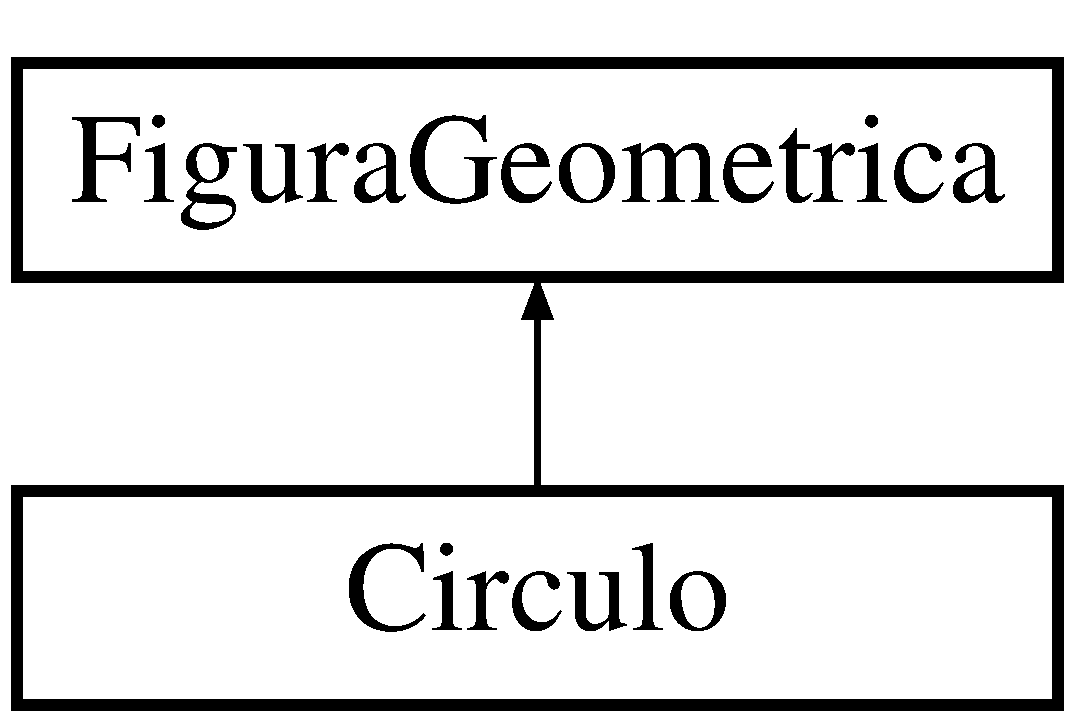
\includegraphics[height=2.000000cm]{class_circulo}
\end{center}
\end{figure}
\subsection*{Public Member Functions}
\begin{DoxyCompactItemize}
\item 
\mbox{\Hypertarget{class_circulo_a3d5f277619ed35f4a8cd455dd1510a20}\label{class_circulo_a3d5f277619ed35f4a8cd455dd1510a20}} 
{\bfseries Circulo} (int \+\_\+x, int \+\_\+y, int raio, int fill)
\item 
void \mbox{\hyperlink{class_circulo_a593787d6e0618c2eded23e8839e7bea6}{draw}} (\mbox{\hyperlink{class_screen}{Screen}} \&t)
\begin{DoxyCompactList}\small\item\em \mbox{\hyperlink{class_circulo_a593787d6e0618c2eded23e8839e7bea6}{Circulo\+::draw}}. \end{DoxyCompactList}\item 
\mbox{\Hypertarget{class_circulo_a197439e429d6636a4a43d77e02b20486}\label{class_circulo_a197439e429d6636a4a43d77e02b20486}} 
void {\bfseries pontos\+Da\+Circunferencia} (int x1, int y1, \mbox{\hyperlink{class_screen}{Screen}} \&t)
\end{DoxyCompactItemize}


\subsection{Member Function Documentation}
\mbox{\Hypertarget{class_circulo_a593787d6e0618c2eded23e8839e7bea6}\label{class_circulo_a593787d6e0618c2eded23e8839e7bea6}} 
\index{Circulo@{Circulo}!draw@{draw}}
\index{draw@{draw}!Circulo@{Circulo}}
\subsubsection{\texorpdfstring{draw()}{draw()}}
{\footnotesize\ttfamily void Circulo\+::draw (\begin{DoxyParamCaption}\item[{\mbox{\hyperlink{class_screen}{Screen}} \&}]{t }\end{DoxyParamCaption})\hspace{0.3cm}{\ttfamily [virtual]}}



\mbox{\hyperlink{class_circulo_a593787d6e0618c2eded23e8839e7bea6}{Circulo\+::draw}}. 


\begin{DoxyParams}{Parameters}
{\em t} & \\
\hline
\end{DoxyParams}
Percorre a extensão do círculo do (centro menos o raio) até o (centro mais o raio) nas direções de x e y, verificando se as coordenadas fornecidas atendem a equação do círculo (x-\/a)² + (y-\/b)² = r². Se o circulo for preenchido, a comparação é feita com a desigualdade $<$=. Se nao, os píxels serão alocados por meio do algoritmo de Bresenham. 

Implements \mbox{\hyperlink{class_figura_geometrica}{Figura\+Geometrica}}.



The documentation for this class was generated from the following files\+:\begin{DoxyCompactItemize}
\item 
circulo.\+h\item 
circulo.\+cpp\end{DoxyCompactItemize}

\hypertarget{class_figura_geometrica}{}\section{Figura\+Geometrica Class Reference}
\label{class_figura_geometrica}\index{Figura\+Geometrica@{Figura\+Geometrica}}
Inheritance diagram for Figura\+Geometrica\+:\begin{figure}[H]
\begin{center}
\leavevmode
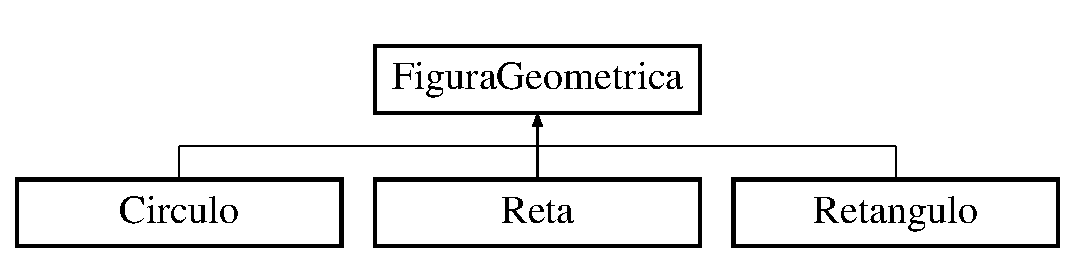
\includegraphics[height=2.000000cm]{class_figura_geometrica}
\end{center}
\end{figure}
\subsection*{Public Member Functions}
\begin{DoxyCompactItemize}
\item 
\mbox{\Hypertarget{class_figura_geometrica_a8ee8dedc060b6059a805ea091aef2c41}\label{class_figura_geometrica_a8ee8dedc060b6059a805ea091aef2c41}} 
virtual void {\bfseries draw} (\mbox{\hyperlink{class_screen}{Screen}} \&t)=0
\end{DoxyCompactItemize}


The documentation for this class was generated from the following files\+:\begin{DoxyCompactItemize}
\item 
figurageometrica.\+h\item 
figurageometrica.\+cpp\end{DoxyCompactItemize}

\hypertarget{class_reta}{}\section{Reta Class Reference}
\label{class_reta}\index{Reta@{Reta}}
Inheritance diagram for Reta\+:\begin{figure}[H]
\begin{center}
\leavevmode
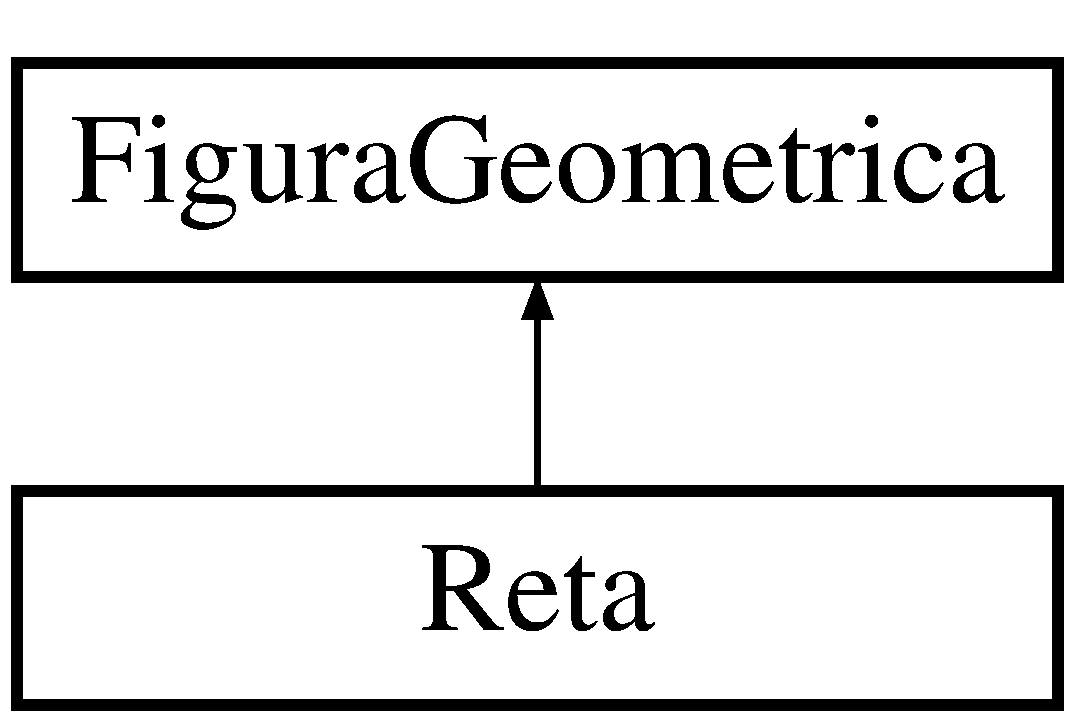
\includegraphics[height=2.000000cm]{class_reta}
\end{center}
\end{figure}
\subsection*{Public Member Functions}
\begin{DoxyCompactItemize}
\item 
\mbox{\Hypertarget{class_reta_aaff4f906cae4e9f8a39d7a356ab8183d}\label{class_reta_aaff4f906cae4e9f8a39d7a356ab8183d}} 
{\bfseries Reta} (int \+\_\+xi, int \+\_\+yi, int \+\_\+xf, int \+\_\+yf)
\item 
\mbox{\Hypertarget{class_reta_ac2e9805183cd474b62bffd8b032cd780}\label{class_reta_ac2e9805183cd474b62bffd8b032cd780}} 
void {\bfseries draw} (\mbox{\hyperlink{class_screen}{Screen}} \&t)
\end{DoxyCompactItemize}


The documentation for this class was generated from the following files\+:\begin{DoxyCompactItemize}
\item 
reta.\+h\item 
reta.\+cpp\end{DoxyCompactItemize}

\hypertarget{class_retangulo}{}\section{Retangulo Class Reference}
\label{class_retangulo}\index{Retangulo@{Retangulo}}
Inheritance diagram for Retangulo\+:\begin{figure}[H]
\begin{center}
\leavevmode
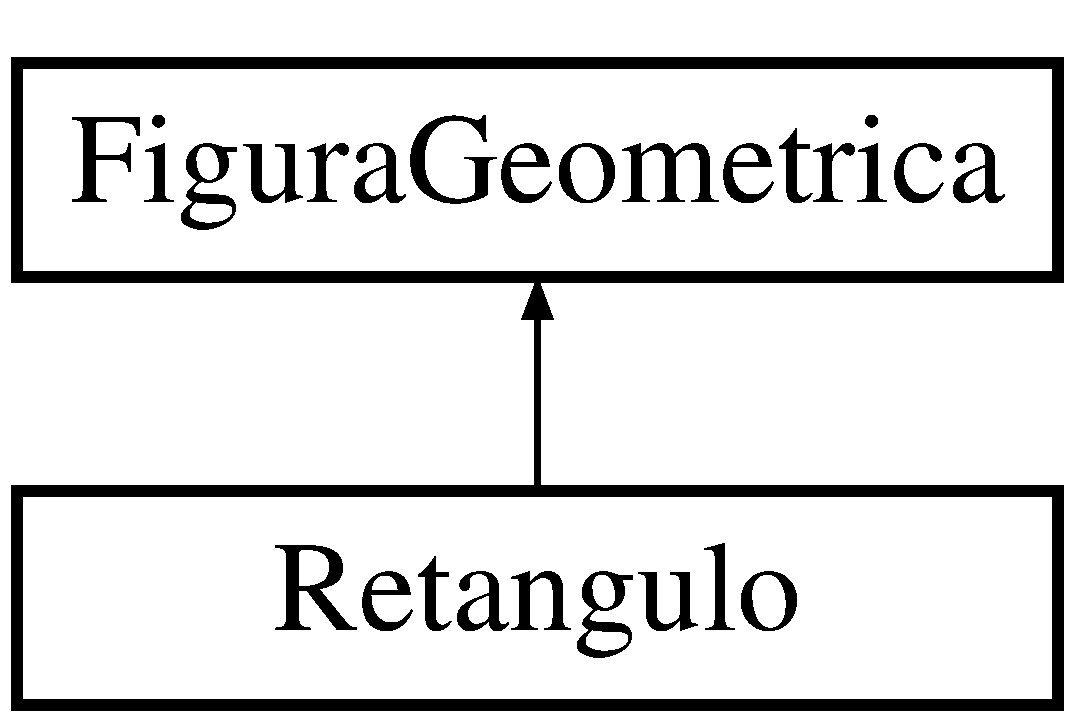
\includegraphics[height=2.000000cm]{class_retangulo}
\end{center}
\end{figure}
\subsection*{Public Member Functions}
\begin{DoxyCompactItemize}
\item 
\mbox{\Hypertarget{class_retangulo_ac971a3083d7f3b268acb5b9373a82c36}\label{class_retangulo_ac971a3083d7f3b268acb5b9373a82c36}} 
{\bfseries Retangulo} (int xc, int yc, int larg, int alt, int fill)
\item 
\mbox{\Hypertarget{class_retangulo_ac088dd6d3f4f3d3f80363a868c2e74f1}\label{class_retangulo_ac088dd6d3f4f3d3f80363a868c2e74f1}} 
void {\bfseries draw} (\mbox{\hyperlink{class_screen}{Screen}} \&t)
\end{DoxyCompactItemize}


The documentation for this class was generated from the following files\+:\begin{DoxyCompactItemize}
\item 
retangulo.\+h\item 
retangulo.\+cpp\end{DoxyCompactItemize}

\hypertarget{class_screen}{}\section{Screen Class Reference}
\label{class_screen}\index{Screen@{Screen}}
\subsection*{Public Member Functions}
\begin{DoxyCompactItemize}
\item 
\mbox{\Hypertarget{class_screen_a246eac542489ef06335800fae60827ee}\label{class_screen_a246eac542489ef06335800fae60827ee}} 
{\bfseries Screen} (int nlin, int ncol)
\item 
\mbox{\Hypertarget{class_screen_ae6bea81c57a22d226507c3c26fa95ee0}\label{class_screen_ae6bea81c57a22d226507c3c26fa95ee0}} 
void {\bfseries set\+Pixel} (int x, int y)
\item 
\mbox{\Hypertarget{class_screen_a35e74266b2a04e37b354ceff7a5f1031}\label{class_screen_a35e74266b2a04e37b354ceff7a5f1031}} 
void {\bfseries clear} ()
\item 
\mbox{\Hypertarget{class_screen_a6fd1e169a3830091a5775a105bcfd1a8}\label{class_screen_a6fd1e169a3830091a5775a105bcfd1a8}} 
void {\bfseries set\+Brush} (char m\+Brush)
\end{DoxyCompactItemize}
\subsection*{Friends}
\begin{DoxyCompactItemize}
\item 
\mbox{\Hypertarget{class_screen_aab6a2880746bfe1b7964817cc8f0989e}\label{class_screen_aab6a2880746bfe1b7964817cc8f0989e}} 
ostream \& {\bfseries operator$<$$<$} (ostream \&os, \mbox{\hyperlink{class_screen}{Screen}} \&t)
\end{DoxyCompactItemize}


The documentation for this class was generated from the following files\+:\begin{DoxyCompactItemize}
\item 
screen.\+h\item 
screen.\+cpp\end{DoxyCompactItemize}

%--- End generated contents ---

% Index
\backmatter
\newpage
\phantomsection
\clearemptydoublepage
\addcontentsline{toc}{chapter}{Index}
\printindex

\end{document}
